%------------------------------------%
%----- 4_Versuchsergebnisse.tex -----%
%------------------------------------%
%------------------------------------%
%
\subsection{Messdaten}
\label{subsec:4_Daten}
%
Zur Bestimmung der Spannung über dem Widerstand $R$ zum Zeitpunkt $t_\mathrm{k}$ wurde die Maschengleichung der Schaltung aufgestellt; der Strom ergab sich aus dem Ohmschen Gesetz am Widerstand $R$:
%
\begin{align*}
   &u_\mathrm{R}(t_\mathrm{k}) = u_\mathrm{E}(t_\mathrm{k}) - u_\mathrm{C}(t_\mathrm{k})
  \numberthis
  \label{eq:4_ur}
  \\
  &i(t_\mathrm{k}) = \frac{u_\mathrm{R}(t_\mathrm{k})}{R}
  \numberthis
  \label{eq:4_i}
\end{align*}
%
Die Messergebnisse sind in Tab. \ref{tab:4_Messdaten} dargestellt\footnote{Alle Werte aufgenommen bzw. berechnet von \autorA}.
%
\begin{table}[H]
  \small
  \centering
	\caption{Messergebnisse}
	\label{tab:4_Messdaten}
	\begin{tabular}{rrrrrr}
	  \toprule
		%
	  \multicolumn{2}{c}{Einstellwerte} &
		\multicolumn{2}{c}{Messwerte} &
		\multicolumn{2}{c}{Berechnete Werte} \\
		\cmidrule(lr{1mm}){1-2}\cmidrule(lr{1mm}){3-4}\cmidrule(lr{1mm}){5-6}
		%
		$t_\mathrm{mess}$ in \si{\micro\second} &
		$t_\mathrm{tat}$ in \si{\micro\second} &
		$u_\mathrm{E}$ in \si{\volt} &
    $u_\mathrm{C}$ in \si{\volt} &
    $u_\mathrm{R}$ in \si{\volt} &
		$i$ in \si{\milli\ampere}\\
		\midrule
		%
		%------------------------------%
    %----- Beginn eures Teils -----%
    %------------------------------%
    %
    \input{src/3_Messwerte.txt}
    % \csvreader[late after line=\\,separator=semicolon]{src/messwertelab1p.csv}{}%
    %{\csvlinetotablerow}%

    %
    \midrule
    %
    % Daten des Ausschaltvorgangs
    %

    %
    %------------------------------%
    %------ Ende eures Teils ------%
    %------------------------------%
    %
		\bottomrule
	\end{tabular}
\end{table}
%
%
%
\newpage
\subsection{Ergebnisplots}
\label{subsec:4_Plots}
%
%------------------------------%
%----- Beginn eures Teils -----%
%------------------------------%
%
\subsubsection{Messung}
\begin{figure}[H]
    \centering
    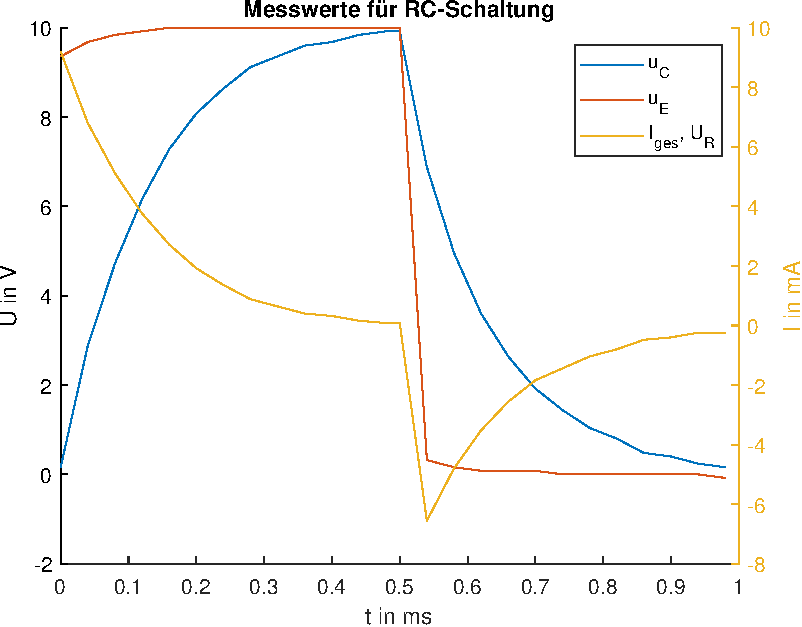
\includegraphics{src/messwerte.pdf}
    \caption{Strom und Spannungverlauft, berechnete plots}
    \label{fig:my_label}
\end{figure}

\subsubsection{Simulation}
\begin{figure}[H]
    \centering
    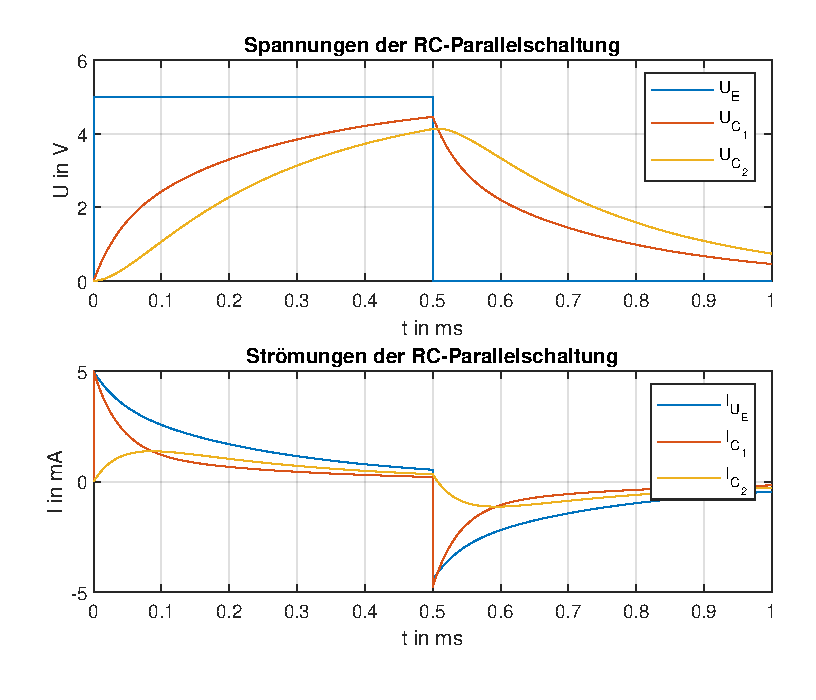
\includegraphics{src/labor2pdf.pdf}
    \caption{Strom und Spannungverlauft, simuliert mit LTSPice}
    \label{fig:my_label2}
\end{figure}
%
%
%
%\begin{flushright}
  %\textit{\autorA}
%\end{flushright}
%
%------------------------------%
%------ Ende eures Teils ------%
%------------------------------%
%
%
%